\documentclass[dvisvgm]{standalone}

\usepackage{tikz}
\usetikzlibrary {arrows.meta, positioning, automata}

\begin{document}

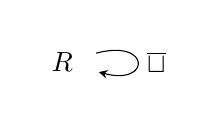
\begin{tikzpicture}[
    ->,
    >=stealth,
    node distance=2cm,
    initial text=$ $,
    on grid,
    every state/.style={fill=none,draw=none}
]

    \node[state]                    (A) {$R$};

    \path
        (A) edge [loop right]       node {$\overline{\sqcup}$}  (A)
    ;
\end{tikzpicture}

\begin{tikzpicture}[
    ->,
    >=stealth,
    node distance=2cm,
    initial text=$ $,
    on grid,
    every state/.style={fill=none,draw=none}
]

    \node[state]                    (A) {$L$};

    \path
        (A) edge [loop right]       node {$\overline{\sqcup}$}  (A)
    ;
\end{tikzpicture}

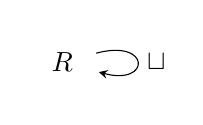
\begin{tikzpicture}[
    ->,
    >=stealth,
    node distance=2cm,
    initial text=$ $,
    on grid,
    every state/.style={fill=none,draw=none}
]

    \node[state]                    (A) {$R$};

    \path
        (A) edge [loop right]       node {$\sqcup$}  (A)
    ;
\end{tikzpicture}

\begin{tikzpicture}[
    ->,
    >=stealth,
    node distance=2cm,
    initial text=$ $,
    on grid,
    every state/.style={fill=none,draw=none}
]

    \node[state]                    (A) {$L$};

    \path
        (A) edge [loop right]       node {$\sqcup$}  (A)
    ;
\end{tikzpicture}

\end{document}